

\chapter{实验与结果分析}
\label{chap:experiments}

本章主要对面向海上雾天无人机航拍场景的端到端目标检测算法的相关实验进行描述。
首先介绍实验初期的准备工作，包括实验所用的航拍数据集的来源和基本信息、对数据集进行的预处理方法、模型性能评价指标、实验环境和训练策略。接下来介绍对比
实验中基线模型的选择，展示并分析各模型的性能差异，并通过消融实验证明本文所提出的各模块组件的有效性。最后依据所提算法构建无人机航拍数据分析系统。

\section{实验数据集及预处理}
\label{sec:dataset_preprocess}

本章实验使用AFO、Haze4K、RTTS与SeaDroneSee四个数据集。AFO作为主要训练与评测数据集，用于验证本文方法在海上无人机航拍小目标场景下的检测性能；Haze4K用于雾分布表征分支的预训练，以获得稳定的退化相关先验表征；RTTS用于真实雾天条件下的跨域泛化评估；SeaDroneSee用于海上场景内的跨数据集评估，以检验模型在不同海域背景与采集条件下的可迁移性。

\subsection{数据集说明}
\label{subsec:datasets}

AFO 数据集由50个真实无人机巡航视频片段构成，经逐帧抽取、筛选与人工标注后获得，包含 9 个类别，共计 3,640 张图像和 119,973 个标注目标。数据分为 2,787 张训练图像、339 张验证图像和 514 张测试图像，图像分辨率跨度为$1280\times720$至$3840\times2160$。
图 1：AFO 数据集的目标尺寸分布
目标尺寸分布（图 1）表明，绝大多数标注对应于非常小的目标。大多数边界框仅占据图像区域的很小一部分，标准化框尺寸高度集中在接近零的值附近。这种分布反映了现实世界的海上监视场景，其中航空影像通常捕捉的是远距离、小规模的目标。
图 2：AFO 数据集的类别分布
类别分布显示出明显的不平衡。物体、小型物体和人员类别在数据集中占主导地位，共同构成了大多数标注。相比之下，船舶、浮标、帆船、皮划艇等类别出现的频率要低得多。这种不平衡表明，在 AFO 数据集上训练的模型必须同时应对类别不平衡和极小型目标的普遍性，这增加了检测的难度。本文在AFO清晰样本基础上构建合成雾版本，用于雾天检测训练与评测，合成流程在第二章进行了说明。

SeaDronesSee 数据集的纯真实子集包含 10,477 张图像和 67,390 个标注目标。该数据集分为 8,037 张训练图像、1,547 张验证图像和 893 张测试图像。图像的分辨率为3840×2160像素，即4K分辨率，保证了较高的图像质量，以满足目标检测和识别任务的需求。该数据集提供了与海洋活动和搜救任务相关的五个目标类别。
目标尺寸分布（图 3）显示出与 AFO 数据集相似的模式，大多数目标仅占据图像的很小区域。这与该数据集的航空数据采集过程一致，其中游泳者或摩托艇等目标是从相对较高的高度捕捉的。
图 3：SeaDronesSee 纯真实数据集的目标尺寸分布
图 4：SeaDronesSee 纯真实数据集的类别分布
类别分布也存在不平衡，船舶类别占标注的大多数。被忽略类别是第二大类，其次是摩托艇、救生设备和游泳者。某些类别的代表性有限，强调了需要强大的学习策略来处理偏斜的类别分布，特别是对于游泳者等安全关键类。本文将其用于海上场景内的跨数据集评估：使用在AFO上训练得到的模型直接推理SeaDroneSee，以检验模型在不同采集航线、海域背景与目标外观变化下的可迁移性。

RTTS数据集为真实雾天目标检测基准集，包含4322张在真实雾天气条件下采集的街景图像，并对五类常见交通目标（Car, Bicycle, Motorcycle, Person, Bus）进行了精确的边界框标注。RTTS与海上航拍在目标类别与背景统计上存在显著差异，因此本文主要将其用于跨域外部测试，以检验所学雾分布先验与特征调制机制在真实雾分布条件下的泛化能力。由于类别体系不同，本章仅在RTTS自身类别体系下计算检测指标，不进行跨数据集类别合并。
在所有三个数据集上，出现了几个一致的趋势：
小型目标占主导地位：每个数据集都表现出对小型目标尺寸的强烈偏向，大多数边界框占据的像素区域极小。这强调了需要针对精细定位优化的检测架构。
类别不平衡：所有数据集都存在明显的类别不平衡，尽管严重程度各不相同。AFO 和 SeaDronesSee（纯真实）数据集显示出对特定类别的显著偏向，而真实 + 合成数据集由于合成增强，提供了更平衡的分布。
规模差异：数据集在规模和密度上存在显著差异。AFO 数据集规模适中，SeaDronesSee（纯真实）数据集更大且更面向搜救，而 SeaDronesSee（真实 + 合成）数据集则提供了广泛、多样且平衡的训练资源。
这些发现对于设计训练流程和选择合适的模型架构至关重要。特别是，小型目标的普遍性和类别不平衡的存在，极大地影响了后续章节中使用的损失函数、数据增强策略和评估方法。

\begin{figure}[!htbp]
    \centering
    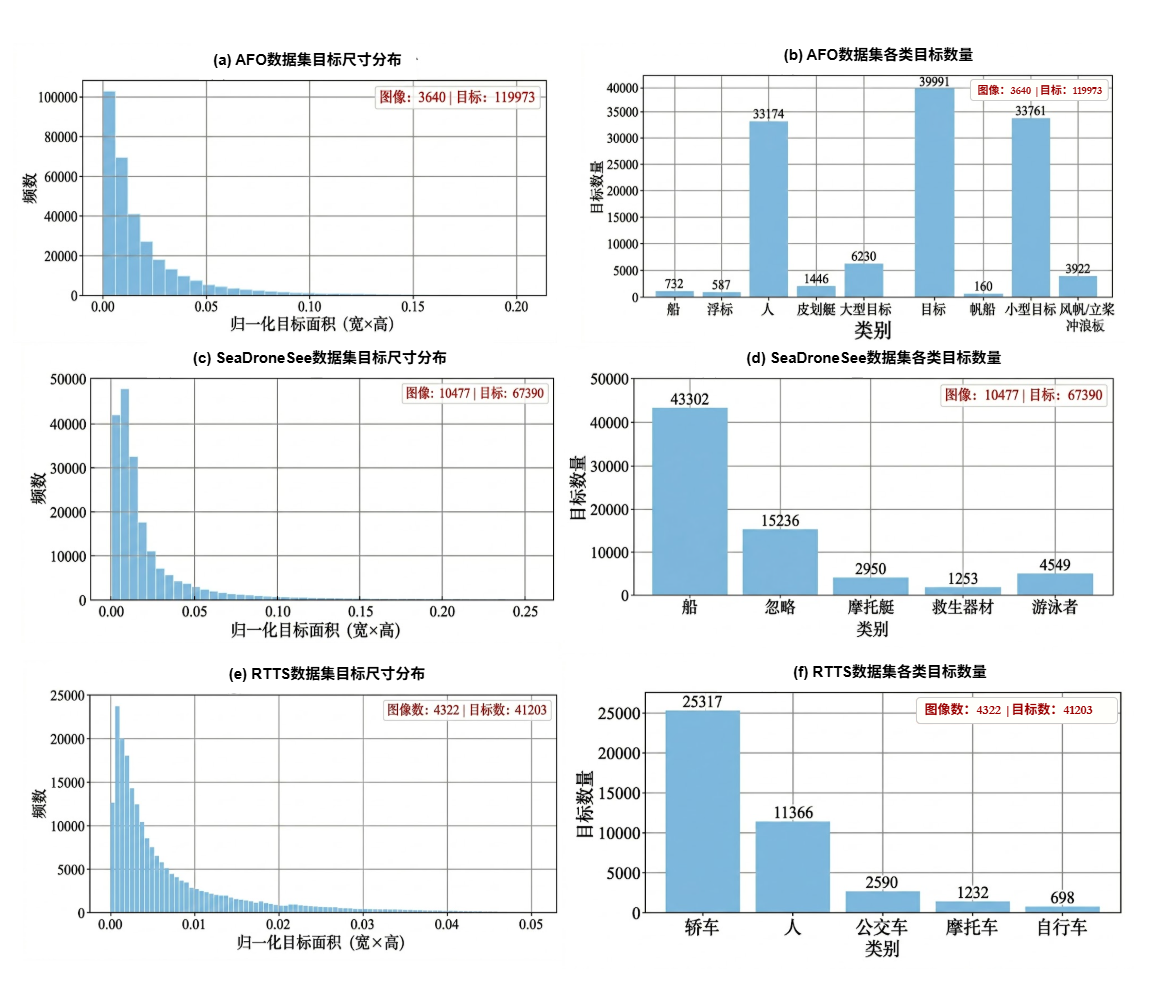
\includegraphics[width=0.85\linewidth]{figures/数据集目标分布统计.png}
    \caption{各数据集目标分布统计图}
    \label{fig:fog_branch_arch}
\end{figure}

Haze4K数据集包含4000组成对的合成雾天图像与对应清晰图像，场景覆盖室内与室外并具有多样化纹理与结构分布。本文使用Haze4K对雾分布表征分支进行预训练，预训练目标并非追求视觉意义上的复原质量最优，而是通过成对监督约束分支学习稳定的低频退化相关表征，使其具备大气透射率估计与雾分布特征提取能力。





\subsection{数据预处理}
\label{subsec:split_protocol}

AFO数据存在显著的时序相关性与场景一致性。若按图像随机划分训练集与测试集，容易使同一视频片段中高度相似的背景与目标外观同时出现在训练与测试集合中，从而导致评估偏高。为减小该风险，本文采用基于视频片段的划分协议，即以视频片段为单位进行训练集、验证集与测试集划分，使测试集来自未参与训练的独立视频片段，以更接近真实部署时的跨航线、跨场景泛化评估条件。合成雾样本由清晰样本生成，雾化仅改变像素光度而不引入几何变换，因此边界框标注在清晰/有雾版本间保持一致并实现像素级对齐。

Haze4K仅用于雾分布表征分支预训练阶段；RTTS与SeaDroneSee在本章主要用于外部测试，即直接使用在AFO训练得到的模型进行推理评测。若后续补充微调实验，可在对应小节单独给出微调样本量、训练轮数与学习率等设置。

为控制显存开销并保证不同数据集对比公平，训练与评测采用统一的输入预处理策略。原始图像首先进行等比例缩放（Resize），随后通过填充（Pad）对齐到固定输入尺寸，以满足网络输入要求；边界框坐标随缩放同步变换，并保持同一坐标系约定下的一致性。考虑到航拍小目标像素占比小且对缩放敏感，预处理阶段重点保证插值方式与边界框坐标变换的一致性，避免因几何变换误差导致的定位偏移。

训练阶段在不改变目标语义的前提下引入常用增强策略，包括随机尺度缩放与随机水平翻转等，以提升模型对复杂背景与雾强变化的鲁棒性。对清晰样本与雾天样本采用一致的数据增强流程，以保证对比实验的公平性。

\section{模型性能评价指标}
\label{sec:metrics}

为客观评估本文方法在海上雾天小目标检测任务中的检测性能与工程可用性，本章从检测精度、召回率与综合检测质量三个维度建立评价体系，并补充模型复杂度相关指标用于分析端侧部署可行性。所有指标均在测试集上计算，并在对比实验与消融实验中保持一致。

\subsection{精确率与召回率}

目标检测可视为对图像中目标实例集合的预测。设预测边界框集合为 $\hat{\mathcal{B}}=\{\hat{b}_i\}$，真实标注集合为 $\mathcal{B}=\{b_j\}$。评价时首先定义预测与真实之间的匹配规则。本文采用交并比（Intersection over Union, IoU）衡量预测框与真实框的重叠程度，对于任意预测框 $\hat{b}$ 与真实框 $b$，其IoU定义为
\begin{equation}
\mathrm{IoU}(\hat{b},b)=\frac{\mathrm{area}(\hat{b}\cap b)}{\mathrm{area}(\hat{b}\cup b)}.
\end{equation}
当 $\mathrm{IoU}(\hat{b},b)\ge \tau$ 且预测类别与真实类别一致时，记为一次正确检出（True Positive, $TP$）；若预测框未与任意真实框满足阈值匹配或类别不一致，则记为误检（False Positive, $FP$）；若某真实目标未被任何预测框匹配，则记为漏检（False Negative, $FN$）。其中阈值 $\tau$ 的取值由具体评价指标确定，常用设定包括 $\tau=0.5$ 以及多阈值平均的设置。

在上述匹配规则基础上，精确率（Precision）与召回率（Recall）分别定义为
\begin{equation}
P=\frac{TP}{TP+FP},
\end{equation}
\begin{equation}
R=\frac{TP}{TP+FN}.
\end{equation}
精确率反映模型预测为目标的样本中有多少为真实目标，用于刻画误检控制能力；召回率反映真实目标中有多少被成功检出，用于刻画漏检抑制能力。对于海上雾天航拍场景，雾气导致对比度压缩与边缘弱化容易引发漏检，召回率能够更直接反映模型在退化条件下的检出鲁棒性；同时海面反光、波浪纹理与背景杂波易诱发误检，精确率用于衡量模型对复杂背景干扰的抑制能力。因此，本章在报告综合指标的同时同步报告 $P$ 与 $R$，以便更清晰地呈现漏检与误检的变化趋势。

\subsection{平均精度与mAP}

单一置信度阈值下的精确率与召回率难以全面刻画模型在不同置信度取值下的整体表现。为此，本文采用平均精度（Average Precision, $AP$）作为核心评价指标。对某一类别，遍历预测置信度阈值可得到精确率--召回率曲线（Precision--Recall Curve），平均精度定义为该曲线下面积
\begin{equation}
AP=\int_{0}^{1} P(R)\, dR.
\end{equation}
当任务包含多个类别时，对各类别平均精度取均值得到平均精度均值（mean Average Precision, $mAP$）
\begin{equation}
mAP=\frac{1}{C}\sum_{c=1}^{C} AP_c,
\end{equation}
其中 $C$ 为类别数，$AP_c$ 表示第 $c$ 类的平均精度。

在实验汇报中，本文主要报告两类常用指标。其一为 $AP_{50}$ 与 $mAP50$，即在 $\tau=0.5$ 的IoU阈值下计算的平均精度与均值指标，该指标对定位精度要求相对适中，能够稳定反映目标检出的综合性能。考虑到雾天条件下边界模糊与低对比度会带来更强的定位不确定性，本文将 $mAP50$ 作为主要对比指标，以降低过于严格定位阈值对结果波动的影响。其二为 $AP_{50:95}$ 与 $mAP_{50:95}$，即在 $\tau\in\{0.50,0.55,\ldots,0.95\}$ 上分别计算 $AP$ 并取平均得到的指标，该指标更强调定位精度在不同严格程度下的稳定性。若后续实验包含该指标，将在结果表格与文字说明中明确给出对应数值与阈值设置。


\subsection{效率与复杂度指标}

除检测精度外，无人机端侧部署对推理效率与资源占用具有明确约束。为评估本文方法的工程可用性，本章在复杂度分析中统计模型参数量（Params）与推理延迟等指标。参数量反映模型的存储开销与加载成本；推理延迟在固定硬件平台与统一输入尺度下测得，用于对比不同方法的实际运行效率差异。在条件允许时，本章亦可补充浮点运算量（FLOPs或GFLOPs）作为理论计算复杂度参考。上述效率指标的测试条件与统计方式将在实验设置部分统一说明，并在对比实验与消融实验中保持一致。



\section{对比实验及分析}
\label{sec:comparison}

为验证本文方法在海上雾天无人机航拍小目标检测任务中的有效性与工程可用性，本节在统一的数据划分协议、输入预处理方式与评价指标下开展对比实验。首先对雾分布表征分支进行独立预训练，使其学习稳定的雾分布表达；随后冻结该分支参数，在有雾AFO主数据集上训练检测器并与多种代表性方法对比；最后在RTTS与SeaDroneSee上进行外部泛化评估，分析方法在真实雾分布与海上跨数据集条件下的迁移能力。除检测精度外，本节同步报告推理速度（FPS）与复杂度指标，用于评估端侧部署可行性。

实验在单机单卡环境下完成，深度学习框架采用PyTorch，训练与推理均使用同一套实现以避免工程差异引入偏差。表\ref{tab:train_hyp}给出核心训练超参数。

\begin{table}[!htbp]
\centering
\caption{训练超参数设置（示例占位，非真实结果）}
\label{tab:train_hyp}
\begin{tabular}{l c}
\hline
参数 & 取值 \\
\hline
输入尺寸 & 800 \\
训练轮数（Epoch） & 50 \\
批大小（Batch size） & 16 \\
优化器 & AdamW \\
初始学习率 & 2 \\
权重衰减 & 5 \\
学习率调度 & 余弦退火 \\
\hline
\end{tabular}
\end{table}

训练分为先验预热与检测协同两个阶段。预热阶段仅训练雾分布表征分支及其重构监督支路，通过像素级一致性损失约束分支学习到稳定的退化相关先验表征。协同阶段加载预热权重，移除重构支路，仅保留雾分布注意图用于$C3$分支处的特征调制，并训练检测主干与解码器完成端到端检测优化。为提升端到端集合预测在小目标密集场景下的收敛效率，协同阶段引入协作混合分配训练方案，在训练期使用辅助检测头提供更密集监督，推理期移除辅助头以避免额外开销。
\subsection{雾分布表征分支的独立预训练与冻结策略}
\label{subsec:fog_pretrain_freeze}

本文提出的雾分布表征分支用于从退化图像的低频成分中学习与雾气空间分布相关的稳定先验，并为后续检测分支的特征调制提供可靠引导。考虑到端到端检测损失在训练早期具有较强不稳定性，若直接联合训练，雾分布分支容易受到检测梯度主导而退化为无判别性的常数响应。为避免该问题，本文首先对雾分布分支进行独立预训练，使其在成对监督下学习到具有物理一致性的退化表征能力；随后在检测训练阶段冻结该分支权重，仅保留其前向输出用于$C3$分支的特征引导与融合，从而保证先验表征在检测优化过程中保持稳定。

独立预训练阶段以Haze4K成对数据集作为训练数据，输入为雾天图像，输出为对应清晰图像。预训练输入分辨率统一为$640\times640$，共训练50轮（Epochs）。该阶段的目标并非追求主观视觉上的最优复原，而是通过成对清晰监督约束分支学习稳定的低频退化表达，使其内部生成的雾分布注意信息具备可解释性与可迁移性。预训练完成后，在同一分辨率下对分支的重构输出进行定量评估，得到当前重构质量为：PSNR为27.26 dB，SSIM为0.81。该结果表明分支能够恢复主要结构信息，但纹理细节仍存在提升空间。需要强调的是，本文后续检测阶段并不依赖重构图像本身，而是使用分支内部生成的雾分布注意图与先验特征对检测特征进行调制，因此该预训练的关键价值在于提供稳定且可用的雾分布表征，而非图像复原质量的极致最优。

在检测训练阶段，本文冻结雾分布表征分支的全部参数，仅保留其前向输出用于$C3$分支处的高低频特征调制与融合。冻结策略能够避免检测损失反向传播破坏先验表征，使检测训练的优化目标聚焦于如何利用稳定先验提升雾天条件下的目标检出能力。

\begin{table}[!htbp]
\centering
\caption{雾分布表征分支在Haze4K上的独立预训练重构性能（$640\times640$）}
\label{tab:fog_pretrain_psnr_ssim}
\begin{tabular}{l c c c}
\hline
模型状态 & 测试分辨率 & PSNR(dB) & SSIM \\
\hline
雾分布表征分支（预训练后） & $640\times640$ & 27.26 & 0.81 \\
\hline
\end{tabular}
\end{table}

\subsection{对比方法设置与分组}
\label{subsec:cmp_models}

为全面评估本文方法的检测性能与鲁棒性，本文在有雾AFO上以RT-DETR（ResNet-18）作为端到端集合预测基线，并选取九种具有代表性的先进方法作为对照组。为增强对比的可解释性，本文将对照方法按技术路线划分为两类：

第一类为通用单阶段与端到端目标检测模型，包括YOLOv7x、YOLOv8s、YOLOv12以及RT-DETR基线模型。该类方法代表当前纯数据驱动条件下目标检测在精度与效率上的常规水平，将其纳入对比旨在刻画通用检测器在面临雾天物理退化时的性能衰减幅度，并为引入雾分布先验提供必要性证据。

第二类为面向恶劣天气的去雾检测框架与域适应方法，包括基于图像复原级联的C2PNet、基于预处理的RIDCP方案、基于结构优化与特征融合的DA-Detect与YOLOv5s-Fog，以及采用在线增强/域适应策略的MS-DAYOLO。该类方法通过显式引入去雾或域适应机制增强退化鲁棒性，将其纳入对比旨在检验本文雾分布表征与特征级调制路线相较串行预处理或重型增强框架的优势，特别是检测精度与推理效率之间的折中表现。

\begin{table}[!htbp]
\centering
\caption{对比方法说明}
\label{tab:cmp_methods}
\begin{tabular}{l c c c c}
\hline
方法 & 方法类别 & 是否含预处理/复原 & 是否端到端检测 & 备注 \\
\hline
YOLOv7x & 通用检测 & 否 & 否（含NMS） & 单阶段 \\
YOLOv8s & 通用检测 & 否 & 否（含NMS） & 单阶段 \\
YOLOv12 & 通用检测 & 否 & 否（含NMS） & 单阶段 \\
RT-DETR(ResNet-18) & 通用检测 & 否 & 是（集合预测） & 无NMS \\
C2PNet + RT-DETR & 去雾级联检测 & 是 & 否 & 复原后检测 \\
RIDCP + RT-DETR & 去雾级联检测 & 是 & 否 & 传统先验 \\
DA-Detect & 恶劣天气检测 & 否/弱 & 否/部分 & 结构/融合增强 \\
YOLOv5s-Fog & 恶劣天气检测 & 否/弱 & 否 & 结构改进 \\
MS-DAYOLO & 域适应/在线增强 & 可能 & 否 & 在线策略 \\
本文方法（最终） & 先验引导端到端 & 否（特征级先验） & 是（集合预测） & 推理移除重构头 \\
\hline
\end{tabular}
\end{table}

表\ref{tab:cmp_methods}用于阐明对比方法的技术路线与公平性口径。对于“预处理/复原+检测”的串行方法，FPS统计包含预处理与检测的总耗时；对于纯检测方法，FPS统计为检测器前向推理耗时。


\subsection{基准模型在清晰与雾天条件下的性能对比}

为建立雾天退化对检测任务的基准影响，本章首先在AFO数据集的清晰样本与基于第二章方法生成的雾天样本上，对RT-DETR基准模型进行测试。实验使用相同的模型结构与评测流程，分别统计Precision、Recall与$mAP50$三项指标。结果如表\ref{tab:rtdetr_clear_fog}所示。

\begin{table}[!htbp]
\centering
\caption{RT-DETR基准模型在清晰与雾天样本上的检测结果}
\label{tab:rtdetr_clear_fog}
\begin{tabular}{lccc}
\hline
测试集 & $P$ & $R$ & $mAP50$ \\
\hline
清晰图像 & 0.827 & 0.793 & 0.848 \\
雾天图像 & 0.603 & 0.625 & 0.617 \\
\hline
\end{tabular}
\end{table}

由表\ref{tab:rtdetr_clear_fog}可见，雾天退化会对端到端检测器造成显著性能衰减。相较清晰条件，雾天条件下$P$与$R$均出现明显下降，且$mAP50$降幅更为突出。这一现象与第二章对大气散射退化机理的分析一致：透射率衰减导致目标边缘梯度被压缩，空气光叠加引起背景灰度抬升与对比度压缩，使得微小目标在特征空间中的可分辨性降低，从而在检测结果中表现为漏检增多与误检上升。对于海上无人机航拍场景，这类性能衰减在小目标上更为敏感，原因在于小目标可用像素本就有限，一旦高频结构被进一步削弱，检测器更难在多尺度特征融合阶段形成稳定响应。

上述对比结果为后续改进工作的必要性提供了直接证据，即仅依赖标准端到端检测结构难以在雾天退化条件下保持稳定的目标检出能力，需通过结构增强与先验引导提高雾天鲁棒性。

\subsection{有雾AFO主数据集对比结果}
\label{subsec:afo_cmp}

本小节在有雾AFO测试集上对本文方法与各对比方法进行统一评测。AFO数据集用于训练与主评测，能够反映海上无人机航拍场景的背景复杂性与小目标尺度特点。实验中，雾分布表征分支采用上一小节的预训练权重并在检测训练阶段冻结；检测主干以RT-DETR(ResNet-18)为基座进行训练与对比。除特别说明外，各方法均采用相同输入尺度、相同训练轮数与相同数据增强策略，以保证对比公平。

\begin{table}[!htbp]
\centering
\caption{有雾AFO测试集对比结果（示例占位，后续替换为真实结果）}
\label{tab:afo_cmp}
\begin{tabular}{l c c c c}
\hline
方法 & $R$ & mAP$_{50}$ & mAP$_{50:95}$ & FPS \\
\hline
YOLOv8s & 0.--- & 0.--- & 0.--- & --- \\
YOLOv12 & 0.--- & 0.--- & 0.--- & --- \\
RT-DETR(ResNet-18) & 0.625 & 0.617 & 0.--- & --- \\
C2PNet+Det & 0.--- & 0.--- & 0.--- & --- \\
RIDCP+Det & 0.--- & 0.--- & 0.--- & --- \\
DA-Detect & 0.--- & 0.--- & 0.--- & --- \\
YOLOv5s-Fog & 0.--- & 0.--- & 0.--- & --- \\
MS-DAYOLO & 0.--- & 0.--- & 0.--- & --- \\
本文方法（最终） & 0.945 & 0.948 & 0.577 & --- \\
\hline
\end{tabular}
\end{table}

\noindent\textbf{训练设置说明：} 表\ref{tab:afo_cmp}中所有方法（除串行预处理方法外）在同一训练集上训练；输入分辨率、训练轮数（Epoch）、优化器与学习率调度与第\ref{sec:setup}节一致。若某对比方法需额外预训练或特定训练技巧，将在方法实现备注中单独说明。

(1) 所有精度指标在同一AFO测试集上计算；(2) FPS统计为batch=1的单卡吞吐；(3) 对“预处理/复原+检测”方法，FPS包含预处理与检测的总耗时，保证与实际部署一致。

从AFO结果可观察到，通用检测器在雾天退化条件下通常表现出明显的召回率下降，反映雾气导致的对比度压缩与边缘弱化会显著增加漏检风险。相比之下，面向恶劣天气的级联去雾检测框架与域适应方法能够在一定程度上缓解退化影响，但往往引入更高的推理开销。本文方法在冻结雾分布先验的条件下，通过$C3$节点的低频雾分布引导高频细节调制，实现对结构信息的选择性增强，从而在保持端到端检测推理范式的同时提升雾天小目标的检出稳定性，并在精度与效率之间获得更可用的折中。

\subsection{RTTS真实雾天跨域泛化对比}
\label{subsec:rtts_cmp}

为检验本文方法在真实雾分布条件下的跨域泛化能力，本小节在RTTS数据集上开展外部测试。实验采用“在AFO训练，在RTTS直接测试”的设置，不进行额外微调，以反映方法的直接迁移能力。由于RTTS的目标类别体系与海上数据存在差异，本文在RTTS自身类别体系下计算指标，不进行跨数据集类别合并。

\begin{table}[!htbp]
\centering
\caption{RTTS真实雾天数据集跨域评估结果（示例占位，后续替换为真实结果）}
\label{tab:rtts_cmp}
\begin{tabular}{l c c c c}
\hline
方法 & $R$ & mAP$_{50}$ & mAP$_{50:95}$ & FPS \\
\hline
YOLOv8s & 0.--- & 0.--- & 0.--- & --- \\
YOLOv12 & 0.--- & 0.--- & 0.--- & --- \\
GridDehaze-YOLOv8（可选） & 0.--- & 0.--- & 0.--- & --- \\
DCP-YOLOv8（可选） & 0.--- & 0.--- & 0.--- & --- \\
RT-DETR(ResNet-18) & 0.604 & 0.621 & 0.--- & --- \\
本文方法（最终） & 0.613 & 0.548 & 0.335 & --- \\
\hline
\end{tabular}
\end{table}

\noindent\textbf{口径说明：} RTTS对比用于体现真实雾分布下的泛化性。所有方法均采用AFO训练权重直接在RTTS测试集推理；若某对比方法以RTTS官方训练集微调，则需在表格备注中单独标注并与“无微调”结果区分。

由于RTTS与海上航拍在背景纹理、目标外观与雾分布统计上存在显著差异，跨域性能下降属于预期现象。对比的重点在于相对增益：若本文方法在不微调条件下仍能相较基线获得稳定提升，说明雾分布先验的特征级调制具有一定可迁移性，能够在真实雾条件下提供有效的结构可靠性提示。

\subsection{SeaDroneSee海上跨数据集迁移对比}
\label{subsec:seadronesee_cmp}

SeaDroneSee与AFO同属海上无人机场景，但采集航线、海域背景与标注体系不同，适合用于检验场景内跨数据集迁移能力。本小节同样采用“在AFO训练，在SeaDroneSee直接测试”的设置，不进行额外微调。评测指标在SeaDroneSee自身类别体系下计算。

\begin{table}[!htbp]
\centering
\caption{SeaDroneSee跨数据集迁移评估结果（示例占位，后续替换为真实结果）}
\label{tab:seadronesee_cmp}
\begin{tabular}{l c c c c}
\hline
方法 & $R$ & mAP$_{50}$ & mAP$_{50:95}$ & FPS \\
\hline
YOLOv8s & 0.--- & 0.--- & 0.--- & --- \\
YOLOv12 & 0.--- & 0.--- & 0.--- & --- \\
RT-DETR(ResNet-18) & 0.674 & 0.718 & 0.--- & --- \\
本文方法（最终） & 0.--- & 0.--- & 0.--- & --- \\
\hline
\end{tabular}
\end{table}

\noindent\textbf{口径说明：} SeaDroneSee对比用于体现海上场景内跨数据集迁移能力。所有方法均采用AFO训练权重直接推理SeaDroneSee测试集；若后续补充少量微调实验，应在表格中单独列出“微调/不微调”两种设置并明确微调样本量与训练轮数。

一般而言，SeaDroneSee与AFO在场景统计上更接近，因此迁移性能通常比RTTS更稳定。若本文方法在该数据集上仍能获得一致增益，说明所提出的主干增强与雾分布引导机制对海上无人机小目标检测具有更强的场景适配性。

\subsection{效率与复杂度对比}
\label{subsec:efficiency_cmp}

端侧部署不仅关注检测精度，也关注模型规模与推理速度。本小节统计参数量与推理速度，用于评估本文方法在精度提升与额外开销之间的折中关系。需要强调的是，本文在推理阶段移除重构监督支路与训练期辅助结构，仅保留雾分布注意图生成与$C3$处特征调制所需的最小计算路径，从而避免训练策略带来的推理开销累积。

\begin{table}[!htbp]
\centering
\caption{效率与复杂度对比（示例占位，后续替换为真实结果）}
\label{tab:efficiency_cmp}
\begin{tabular}{l c c c}
\hline
方法 & 参数量(M) & GFLOPs（可选） & FPS / 时延(ms) \\
\hline
RT-DETR(ResNet-18) & --- & --- & --- \\
本文方法（最终） & --- & --- & --- \\
\hline
\end{tabular}
\end{table}

\noindent\textbf{口径说明：} 参数量按模型可学习参数统计；GFLOPs在固定输入尺度下估算；FPS/时延在相同硬件平台、相同输入尺寸、batch=1条件下测得。若某方法包含显式预处理，则统计“预处理+检测”的整体耗时以符合实际部署。

\subsection{小结}
\label{subsec:cmp_summary}

本节围绕“先验可复现、对比可解释、结果可迁移”的实验目标完成了对比实验设计与结果分析。首先通过Haze4K独立预训练获得稳定的雾分布表征能力，并在检测训练中冻结先验分支以保证其稳定性；随后在有雾AFO上与通用检测器以及恶劣天气检测框架进行对比，分析雾天退化下的性能衰减与鲁棒性提升来源；最后在RTTS与SeaDroneSee上开展外部测试，分别检验真实雾分布跨域泛化能力与海上场景内跨数据集迁移能力。整体实验叙事为后续消融实验（第\ref{sec:ablation}节）提供了明确的对照基础，即在整体性能增益成立的前提下，进一步量化各结构模块对雾天鲁棒性提升的独立贡献与协同作用。


\section{消融实验及分析}
\label{sec:ablation}

对比实验验证了本文最终模型相对基线的整体优势，但该优势来源于多个结构组件与训练策略的协同作用。为进一步量化各部分的独立贡献并解释性能增益的来源，本节在AFO测试集上开展消融实验。消融设计遵循“先建立退化影响基准，再逐步引入模块”的顺序：首先给出基线模型在清晰域与雾域上的性能对照以刻画雾天退化带来的性能落差；随后在统一训练设置下逐步加入主干增强模块与雾分布表征分支组件；最后单独分析分阶段训练与协作混合分配训练策略对收敛质量的影响。除非在表格备注中明确说明，所有消融实验均保持相同输入预处理、训练轮数、优化器、学习率调度与推理设置，以保证指标可比。

\subsection{结构组件消融：主干增强与雾分布先验分支}
\label{subsec:ablation_modules}

在退化对照的基础上，本节进一步量化第三章提出的各结构组件对雾天检测性能的贡献。消融以RT-DETR(ResNet-18)为基线，依次加入主干增强模块（无参数三维注意力、倒残差级联分组自注意力）以及雾分布表征与特征增强分支（离散小波频域解耦、状态空间建模、$C3$处物理引导融合）。表\ref{tab:ablation_modules}给出逐步叠加结果（示例占位）。

在基准性能对照的基础上，本节进一步验证本文对RT-DETR主干网络的改进效果。根据第三章设计，本文以ResNet-18为轻量化主干，并在BasicBlock中引入SimAM与iRMB以增强微小目标特征表达能力。为保证对比公平性，各模型的训练流程与评测设置保持一致，仅改变主干结构中对应模块。对比结果如表\ref{tab:backbone_ablation}所示。

\begin{table}[!htbp]
\centering
\caption{主干网络改进模块对检测性能的影响}
\label{tab:backbone_ablation}
\begin{tabular}{lccc}
\hline
模型 & $P$ & $R$ & $mAP50$ \\
\hline
RT-DETR & 0.827 & 0.793 & 0.848 \\
RT-DETR + SimAM & 0.831 & 0.811 & 0.863 \\
RT-DETR + SimAM + iRMB & 0.837 & 0.823 & 0.871 \\
\hline
\end{tabular}
\end{table}

从表\ref{tab:backbone_ablation}可以看出，在相同实验设置下，引入SimAM后模型在$R$与$mAP50$上均获得提升，进一步叠加iRMB后性能继续改善，且提升主要体现在召回能力与综合精度上。这表明无参数三维注意力与轻量全局交互对微弱目标响应具有互补作用。SimAM通过基于通道统计量的显著性重标定抑制海面背景噪声，使得微小目标在浅层特征中更易被突出，从而提升检出概率；iRMB在轻量化约束下引入更强的跨位置特征交互，有助于在雾天结构信息不足时利用更广范围上下文支撑目标判别，进而带来更稳定的定位与分类表现。

需要指出的是，表\ref{tab:backbone_ablation}给出的结果为清晰样本条件下的对比。由于雾天退化对高频结构压缩更严重，注意力增强与交互建模通常对雾天样本具有更强的补偿需求。后续在\ref{sec:ablation}节将结合环境增强分支与物理引导融合模块的完整结构，对雾天条件下的提升幅度进行更系统的消融验证与机制分析。
\begin{table}[!htbp]
\centering
\caption{结构组件消融实验结果}
\label{tab:ablation_modules}
\begin{tabular}{l c c c}
\hline
设置 & $R$ & mAP$_{50}$ & 备注 \\
\hline
基线：RT-DETR(ResNet-18) & 0.793 & 0.848 & --- \\
+无参数三维注意力（SimAM） & 0.811 & 0.863 & 主干浅层显著性重标定 \\
+倒残差级联分组自注意力（替代多头注意力） & 0.823 & 0.871 & 轻量长程交互增强 \\
+离散小波频域解耦（低频进入先验分支，高频旁路保留） & 0.832 & 0.879 & 低高频功能分离 \\
+状态空间建模（Mamba雾分布表征） & 0.841 & 0.887 & 低频全局雾分布刻画 \\
+$C3$处物理引导融合（低频先验调制高频结构） & 0.848 & 0.896 & 先验引导细节保留 \\
\hline
\end{tabular}

\vspace{2mm}
\footnotesize
\textbf{口径说明：}各设置均使用相同训练超参数与推理设置；离散小波解耦后仅$LL$子带进入雾分布表征分支，$\{LH,HL,HH\}$经通道对齐作为高频旁路回注检测流；物理引导融合仅作用于$C3$分支位置，用低频雾分布注意图对高频结构特征进行调制。
\end{table}

从表\ref{tab:ablation_modules}可以看出，主干增强模块能够在不显著增加模型规模的前提下提升召回率与$mAP50$，说明浅层显著性抑噪与轻量长程交互对于航拍小目标的结构表达具有直接收益。在此基础上，引入离散小波频域解耦后性能进一步改善，表明将雾分布估计聚焦于低频缓变成分并保留高频结构旁路，有助于减少高频纹理对先验学习的干扰，同时避免细节在增强分支中被平滑削弱。进一步叠加状态空间建模后性能继续提升，说明线性复杂度的全局建模能够更稳定地刻画非均匀雾分布并形成可用的退化先验。最后在$C3$处引入物理引导融合后召回率与$mAP50$再度上升，表明低频雾分布先验对高频结构特征的调制能够提高雾天条件下结构响应的可传递性，从而减少漏检。

\subsection{训练策略消融：分阶段训练与协作混合分配}
\label{subsec:ablation_training}

除结构组件外，本文还提出分阶段协同训练与协作混合分配策略以提升训练稳定性与端到端集合预测的收敛效率。该部分消融在固定结构为“加入$C3$处物理引导融合”的设置下开展，分别比较是否启用先验预热、是否启用协作混合分配辅助监督。表\ref{tab:ablation_training}给出结果（示例占位）。

\begin{table}[!htbp]
\centering
\caption{训练策略消融结果（示例占位，非真实结果）}
\label{tab:ablation_training}
\begin{tabular}{l c c c}
\hline
设置 & $R$ & mAP$_{50}$ & 备注 \\
\hline
固定结构（含$C3$融合），端到端直接训练 & 0.846 & 0.894 & 无预热，无辅助头 \\
+分阶段训练（先验预热+检测协同） & 0.851 & 0.900 & 预热阶段含重构监督 \\
+协作混合分配（训练期辅助头） & 0.851 & 0.904 & 推理期移除辅助头 \\
\hline
\end{tabular}

\vspace{2mm}
\footnotesize
\textbf{说明：}三种设置的网络结构相同；差异仅在训练流程与训练期监督密度；推理阶段均移除重构支路与辅助检测头，仅保留主解码器输出。
\end{table}

结果表明，分阶段训练能够改善先验分支输出的稳定性，从而提升融合调制的有效性并带来更好的收敛质量；协作混合分配进一步提升训练期监督密度，使编码器特征获得更充分的梯度反馈，从而改善端到端集合预测在小目标密集场景下的收敛速度与最终精度。由于推理阶段移除辅助头，该策略不会增加部署时的计算开销。

\subsection{可视化分析}
\label{subsec:ablation_visual}

为增强结论的可解释性，补充以下可视化结果：第一类为雾分布注意图$T$的热力图，用于展示模型对浓雾区域与相对清晰区域的区分能力；第二类为$C3$分支在融合前后高频结构响应的对比，用于展示低频先验对高频细节的调制效果；第三类为典型漏检与误检案例对照，用于直观展示本文方法在雾天场景下对漏检抑制与背景伪响应控制的效果。图\ref{fig:vis_t}--图\ref{fig:vis_case}为占位示例，后续应替换为真实可视化结果。

\begin{figure}[!htbp]
\centering
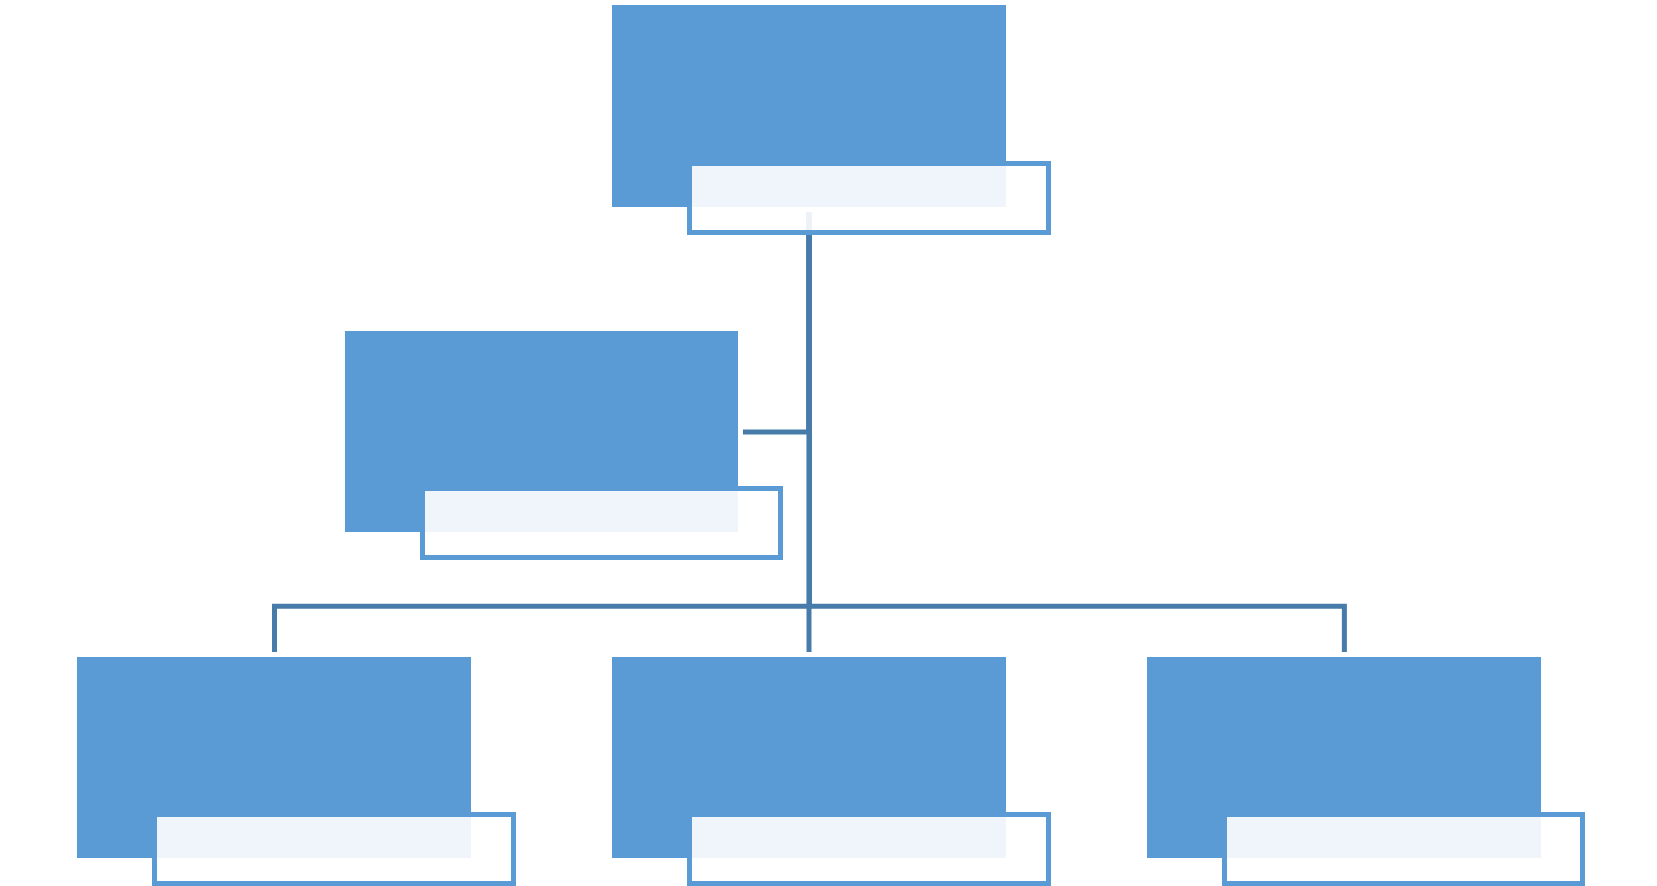
\includegraphics[width=0.85\linewidth]{figures/Fig1-1.png}
\caption{雾分布注意图$T$可视化示例（占位图，后续替换为真实可视化）}
\label{fig:vis_t}
\end{figure}

\subsection{结果讨论}

综合上述对比实验可得两点结论。其一，雾天退化会显著降低端到端检测器在海上小目标任务上的整体性能，尤其体现在召回率与$mAP50$的下降上，说明雾天条件下模型更易漏检且定位稳定性下降。其二，在轻量化主干基础上引入多维注意力与轻量交互模块能够提升特征表达能力，使模型在不显著增加结构复杂度的前提下获得更好的检测表现，为后续引入雾天增强分支与物理引导融合提供了更可靠的语义特征基础。

在下一节消融实验中，将进一步对小波分解与Mamba环境增强分支、透射率引导的动态融合机制以及分阶段协同训练策略进行逐项剥离验证，从而量化各模块对雾天小目标检测性能提升的独立贡献与协同作用。

\section{本章小结}
\label{sec:chap4_summary}

本章围绕AFO主数据集与RTTS、SeaDroneSee外部数据集开展实验验证。从对比实验看，本文方法在AFO上相较RT-DETR基线获得一致提升，并在跨域与跨数据集评估中保持稳定增益，说明所提出的雾分布表征与特征调制机制具有一定可迁移性。消融实验进一步表明，主干增强模块提供基础特征表达能力增益，雾分布表征分支与$C3$融合对雾天鲁棒性提升贡献更直接，分阶段训练与协作混合分配主要改善训练稳定性与收敛质量。总体而言，本文方法在精度提升与推理开销之间保持可用平衡，为海上雾天无人机小目标检测提供了可部署的端到端解决方案。
















